Recordando a Segunda Lei de Fick mencionada na seção \ref{sec:difusao}, estuda-se uma solução numérica para a equação diferencial eq.(\ref{eq:2alei-num}).

\begin{equation}
\label{eq:2alei-num}
\pdv{C(x,t)}{t} = D(C)\pdv[2]{C(x,t)}{x} \;.
\end{equation}

Para essa solução, considera-se o coeficiente de difusão constante (independente da concentração, D(C) = D. Utilizando o método das diferenças finitas apresentado na seção \ref{sec:dif-fin}, a discretização do espaço será dada por um espaçamento {$\Delta x$}, e representa-se por $i$ o i-ésimo nó do eixo x. Para o passo do tempo, utilizou-se um passo {$\Delta t$}, e $j$ nota o j-ésimo instante de tempo. Assim, tem-se a representação discretizada da eq.(\ref{eq:2alei-num}) dada pela eq.(\ref{eq:2alei-discr}) e um esquema dessa malha ilustrado na Figura \ref{fig:malha}. Destaca-se que foi utilizado o método implícito das diferenças finitas para essa parte do trabalho.

\begin{equation}
\label{eq:2alei-discr}
\dfrac{C_i^{j+1} - C_i^j}{\Delta t} = D\dfrac{C_{i+1}^{j+1} - 2C_i^{j+1} + C_{i-1}^{j+1}}{(\Delta x)^2}  \;.
\end{equation}



\begin{figure}[ht]
	\caption{Malha de discretização}
	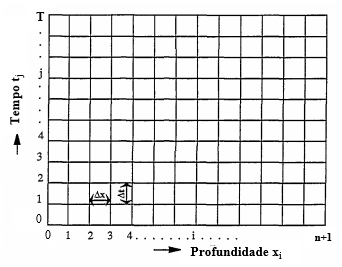
\includegraphics{malha}
	\label{fig:malha}
	\centering
    \fonte{adaptado de Y.Sun; T.Bell, 1997}	
	\end{figure}


As condições de contorno adotadas serão as mesmas apresentadas na seção \ref{sec:difusao}, isto é, a concentração inicial de nitrogênio no interior do material é nula e a concentração na superfície se mantém constante ao longo do tempo. Essas condições podem ser descritas da seguinte forma:

\begin{gather*}
		\mathrm{Condição\ Inicial: }\ C(x, t=0) = c_i^0 = 0 \qquad i \in [0;\ n+1] \;. \\
		\mathrm{Condições\ de\ Contorno:}\ 
		\left\{
    		\begin{array}{l}
      			C(x=0, t>0) = C_0^j = C_s  \\
				C(x\rightarrow\infty, t>0) = C_{n+1}^j = 0 
			\end{array}
    		\begin{array}{l}
      		\qquad \\
			\qquad \\	   
    		\end{array}
    		\begin{array}{l}
    			j \in [0,\ T] \;.
    		\end{array}
		\right.	
\end{gather*}


A eq.(\ref{eq:2alei-discr}) pode ser reescrita como:

\begin{equation}
\label{eq:antesFo}
C_i^{j+1} - \frac{D\Delta t}{(\Delta x)^2} (C_{i+1}^{j+1} - 2C_i^{j+1} + C_{i-1}^{j+1}) = C_i^j \;.
\end{equation}

A relação $\dfrac{D\Delta t}{(\Delta x)^2}$ é um número adimensional chamado de número de Fourier. Seja $Fo = \dfrac{D\Delta t}{(\Delta x)^2} $, a eq.(\ref{eq:antesFo}) é reescrita subsitituindo com $Fo$, isolando a incógnita ao lado esquerdo:

\begin{gather*}
\label{eq:depoisFo}
- FoC_{i+1}^{j+1} + (1+2Fo)C_i^{j+1} - FoC_{i-1}^{j+1} = C_i^j \\
C_i^{j+1} = \dfrac{1}{(1+2Fo)}C_i^j + \dfrac{Fo}{(1+2Fo)}C_{i-1}^{j+1} + \dfrac{Fo}{(1+2Fo)}C_{i+1}^{j+1} \;.
\end{gather*}

Segundo o critério de estabilidade mencionado na seção \ref{sec:dif-fin}, como $Fo>0$, o esquema implícito é sempre estável.

Agora desenvolve-se o sistema de equações para resolver o problema diferencial.

\begin{equation*}
\label{eq:depoisFo}
\begin{matrix}
i = 1: \qquad & -FoC_{0}^{j+1}   & + & (1+2Fo)C_1^{j+1} & - & FoC_{2}^{j+1} & - & C_1^j & = & 0\\
              &&&&& (1+2Fo)C_1^{j+1} & - & FoC_{2}^{j+1} & = & FoC_{s}^{j+1}  + C_1^j \\ 
\\
i = 2: \qquad & -FoC_{1}^{j+1} & + & (1+2Fo)C_2^{j+1} & - & FoC_{3}^{j+1} & - & C_2^j & = & 0\\
              &&& (1+2Fo)C_2^{j+1} & - & FoC_{3}^{j+1} & - & FoC_{1}^{j+1} & = & C_2^j \\ 
\vdots \\
i = n: \qquad & -FoC_{n-1}^{j+1} & + & (1+2Fo)C_n^{j+1} & - & FoC_{n+1}^{j+1} & - & C_n^j & = & 0\\
              &&&&& (1+2Fo)C_n^{j+1} & - & FoC_{n-1}^{j+1} & = & C_n^j \\ 
\end{matrix}
\end{equation*}

Seja o sistema de equações dado por \cmrtext{AC$^{j+1}$ = B$^j$}, \cmrtext{A, C e B} podem ser definidos por:

\begin{equation*}
	\cmrtext{A} =
	\begin{bmatrix}
		(1+2Fo) & -Fo &   0    &  \ldots   & 0\\
		-Fo & (1+2Fo) &  -Fo   &        & \vdots \\
		 0  & -Fo &   (1+2Fo)   & \ddots & \vdots\\
	 \vdots &     &  \ddots & \ddots & -Fo \\
	     0  & \ldots  &  \ldots &  -Fo   & (1+2Fo) 
	\end{bmatrix}
\end{equation*}
\begin{equation*}
	\cmrtext{C^{j+1}} =
	\begin{bmatrix}
		c_1^{j+1} \\
		c_2^{j+1} \\
		c_3^{j+1} \\
		\vdots \\
		c_n^{j+1}
	\end{bmatrix}
	\qquad
	\cmrtext{B^j} =	
	\begin{bmatrix}
		Fo\ c_s+c_1^j \\
		c_2^{j} \\
		c_3^{j} \\
		\vdots \\
		c_n^{j}
	\end{bmatrix}
\end{equation*}

\cmrtext{A} é uma matriz tridiagonal, \cmrtext{AC$^{j+1}$ = B$^j$} é um sistema de $n$ equações lineares com $n$ incógnitas. Logo, pode-se utilizar o algoritmo de Thomas visto na seção \ref{sec:algo-thomas} para solucionar o problema.